\documentclass[runningheads]{llncs}

% ---- Packages ----
\usepackage[T1]{fontenc}
\usepackage{graphicx}
\usepackage{amsmath,amssymb}
\usepackage{booktabs}
\usepackage{multirow}
\usepackage{hyperref}
\usepackage{xcolor}
\usepackage{subcaption}
\usepackage[nocompress]{cite}

\begin{document}

\title{Explainable Multi-Label Chest Pathology Detection\\
via Asymmetric Loss and Grad-CAM Visualization}

\author{Zeeshan Modi\inst{1}}

\authorrunning{Z. Modi}

\institute{
  University of Bremen, Bremen, Germany\\
  \email{zeeshan.modi@uni-bremen.de}
}

\maketitle

% ================================================================
\begin{abstract}
Chest radiograph interpretation is one of the most demanding and
time-intensive tasks in routine radiology. This paper presents
\textbf{MedVision-AI}, a deep learning framework for simultaneous
detection of 14 thoracic pathologies from chest X-rays. We train
a DenseNet-121 backbone with Asymmetric Loss (ASL) on the NIH
ChestX-ray14 dataset, which comprises 112,120 frontal-view images
and presents substantial class imbalance across its 14 disease
categories. To make model decisions transparent to clinicians, we
incorporate Grad-CAM visualizations that produce class-specific
attention maps over the input image. A controlled backbone
comparison against ResNet-50 under identical training conditions
shows that DenseNet-121 achieves a mean AUC of 0.7978, compared
to 0.7067 for ResNet-50 and 0.7380 reported by Wang et~al.
Additionally, we release a Gradio-based web interface that allows
practitioners to upload chest X-rays and receive predictions with
visual explanations in real time.
\end{abstract}

\keywords{Chest X-ray \and Multi-label classification \and
Grad-CAM \and Explainable AI \and Asymmetric Loss \and
Thoracic pathology detection}

% ================================================================
\section{Introduction}
\label{sec:intro}

Chest radiography remains the most frequently ordered imaging
examination in clinical medicine. In many healthcare settings,
particularly in low- and middle-income countries, the number of
radiographs far exceeds the capacity of available
specialists~\cite{wang2017chestxray14}. Automated computer-aided
detection systems trained on large annotated datasets offer a
practical path toward closing this gap, provided they are both
accurate and interpretable enough to support clinical decision-making.

The NIH ChestX-ray14 dataset~\cite{wang2017chestxray14} has become
the standard benchmark for this problem. It contains over 112,000
frontal chest radiographs labeled with up to 14 co-occurring
pathologies, extracted from radiology reports using natural
language processing. This multi-label structure means that any
given image may be positive for several conditions simultaneously,
while certain pathologies such as Hernia and Pneumonia appear in
fewer than one percent of cases. Standard cross-entropy loss
treats all samples equally regardless of label frequency, which in
practice causes models to suppress predictions for rare classes
entirely. Addressing this imbalance is therefore central to
achieving reliable detection across all 14 categories.

Beyond accuracy, clinical deployment of AI systems for radiology
requires that predictions be explainable. A model that outputs
high confidence for Pneumothorax without indicating where in the
image that evidence lies is of limited value to a radiologist.
Grad-CAM~\cite{selvaraju2017gradcam} solves this by computing
class-specific importance maps from the gradients of the predicted
class score with respect to the final convolutional feature maps.
No changes to the model architecture are needed, making it easy
to apply to any trained convolutional network.

In this work, we make the following contributions:
\begin{itemize}
  \item We conduct a head-to-head backbone comparison between
        ResNet-50 and DenseNet-121, trained under identical
        conditions with Asymmetric Loss, and show that
        DenseNet-121 achieves 9.1 percentage points higher
        mean AUC on the official ChestX-ray14 test set.
  \item We show that Asymmetric Loss successfully prevents
        the class-collapse behavior that ResNet-50 exhibits
        on the three most prevalent positive classes when
        trained with standard binary cross-entropy.
  \item We integrate Grad-CAM to generate per-class heatmaps
        and demonstrate that the model's spatial attention
        aligns with known radiological landmarks for several
        pathologies.
  \item We release all code, evaluation scripts, and a Gradio
        interface at \url{https://github.com/Zeesejo/medvision-ai}.
\end{itemize}

% ================================================================
\section{Related Work}
\label{sec:related}

\paragraph{Multi-label chest X-ray classification.}
Wang et al.~\cite{wang2017chestxray14} introduced the ChestX-ray14
benchmark alongside a DenseNet-121 baseline, establishing per-class
AUC scores that have since served as the reference point for
comparison. CheXNet~\cite{rajpurkar2017chexnet} demonstrated that
a deeper DenseNet trained with careful tuning could match or exceed
radiologist performance on pneumonia detection within the same
dataset. Later work explored attention-guided training to
improve localization~\cite{chen2019attention} and graph
convolutional networks to model label
correlations~\cite{chen2019gcn}. More recently, transformer-based
architectures~\cite{dosovitskiy2020vit,ma2021vit} have pushed mean
AUC values on ChestX-ray14 into the 0.83 to 0.85 range, primarily
through better modeling of long-range spatial dependencies.

\paragraph{Handling class imbalance.}
Focal Loss~\cite{lin2017focal} was originally proposed for object
detection and down-weights the loss contribution of easy negative
examples. Asymmetric Loss~\cite{ridnik2021asl} refines this idea
by applying separate focusing parameters to positive and negative
predictions, combined with a probability margin that hard-thresholds
near-zero negative predictions to zero. This asymmetry consistently
benefits multi-label recognition, particularly for rare categories,
and has shown strong results across MS-COCO and Pascal VOC.

\paragraph{Visual explanations.}
Grad-CAM~\cite{selvaraju2017gradcam} produces class-discriminative
localization maps by weighting the activations of the final
convolutional layer by the corresponding class gradient. It has
been widely adopted in medical imaging as a lightweight
interpretability tool, and several studies have validated its
anatomical alignment against radiologist annotations for pathologies
such as Cardiomegaly, Effusion, and Pneumothorax.

% ================================================================
\section{Methodology}
\label{sec:method}

\subsection{Dataset}
We use the NIH ChestX-ray14 dataset~\cite{wang2017chestxray14},
which contains 112,120 frontal chest X-rays from 30,805 unique
patients annotated with 14 thoracic disease labels. We follow the
official patient-level train/test split to prevent data leakage,
yielding 77,872 training images, 8,652 validation images, and
25,596 test images. During training, images are randomly cropped
to 224 by 224 pixels, horizontally flipped with probability 0.5,
and subjected to mild color jitter. At evaluation time all images
are resized to 320 by 320 pixels.

\subsection{Model Architecture}
Two backbone architectures are evaluated under identical conditions.

\paragraph{ResNet-50.}
A 50-layer residual network~\cite{he2016resnet} pretrained on
ImageNet, producing a 2048-dimensional global average-pooled
feature vector.

\paragraph{DenseNet-121.}
A 121-layer densely connected network~\cite{huang2017densenet}
pretrained on ImageNet with 7.5 million parameters, producing a
1024-dimensional feature vector. Dense connectivity means every
layer receives direct input from all preceding layers within a
block, which encourages feature reuse and provides denser gradient
flow during backpropagation.

Both backbones feed into an identical classification head:
\begin{equation}
  \hat{y} = \sigma\!\left( W_2 \cdot \text{GELU}(W_1 \cdot
  \text{LN}(\mathbf{z})) \right)
  \label{eq:head}
\end{equation}
where $\text{LN}$ is Layer Normalization, dropout with $p = 0.3$
is applied after the hidden layer, and $\sigma$ denotes the
sigmoid function applied independently to each of the 14 outputs.

\subsection{Loss Function}
We train with Asymmetric Loss~\cite{ridnik2021asl}:
\begin{equation}
  \mathcal{L}_{\text{ASL}} = -\frac{1}{N}\sum_{i}\sum_{c}
  \Bigl[ y_{ic}\,(1-p_{ic})^{\gamma^+}\log p_{ic} +
  (1-y_{ic})\,(p^-_{ic})^{\gamma^-}\log(1-p^-_{ic}) \Bigr]
  \label{eq:asl}
\end{equation}
where $p^-_{ic} = \max(p_{ic} - m, 0)$ shifts near-zero negative
predictions to exactly zero using a margin $m = 0.05$, and the
focusing exponents are set to $\gamma^+ = 0$ and $\gamma^- = 4$.
The asymmetric design places stronger down-weighting on easy
negative examples while leaving positive gradient contributions
relatively unattenuated, which is well suited to the severe
positive-negative imbalance in ChestX-ray14.

\subsection{Training Protocol}
Both models are trained for 30 epochs using
AdamW~\cite{loshchilov2019adamw} with a learning rate of $10^{-4}$
and weight decay $10^{-4}$. The learning rate follows a cosine
annealing schedule with 3 linear warmup epochs. Gradients are
clipped to unit $\ell_2$ norm, and automatic mixed precision (AMP)
is used throughout. Early stopping monitors validation mean AUC
with a patience of 7 epochs. The best checkpoint by validation AUC
was reached at epoch 15 for ResNet-50 and epoch 30 for DenseNet-121.

\subsection{Grad-CAM}
For each class $c$, Grad-CAM computes importance weights by global
average pooling the gradients of $y^c$ over the spatial dimensions
of the final convolutional feature maps $A^k$:
\begin{equation}
  \alpha_k^c = \frac{1}{Z}\sum_i\sum_j
  \frac{\partial y^c}{\partial A^k_{ij}}
  \label{eq:gradcam_weights}
\end{equation}
The class activation map is then obtained by a weighted sum of
feature maps passed through a ReLU:
\begin{equation}
  L^c = \text{ReLU}\!\left(\sum_k \alpha_k^c A^k \right)
  \label{eq:gradcam_map}
\end{equation}
For DenseNet-121 we extract gradients at the output of
\texttt{denseblock4}; for ResNet-50 at \texttt{layer4}. The
resulting maps are bilinearly upsampled to the input image size
and overlaid as a color heatmap.

% ================================================================
\section{Experiments}
\label{sec:experiments}

\subsection{Evaluation}
Following Wang et al.~\cite{wang2017chestxray14}, we report the
area under the ROC curve (AUC) for each pathology class on the
official test split of 25,596 images, and summarize performance
with the unweighted mean AUC across all 14 classes.

\subsection{Results}

Table~\ref{tab:auc} reports per-class and mean AUC for both
models alongside the Wang et al.\ baseline. DenseNet-121 with
Asymmetric Loss achieves a mean AUC of 0.7978, which is 6.0
points above the Wang et al.\ reference (0.7380) and 9.1 points
above our ResNet-50 run (0.7067). The largest absolute gains
relative to the baseline are observed for Emphysema (0.916),
Hernia (0.891), Pneumothorax (0.857), and Cardiomegaly (0.869),
all of which correspond to pathologies with visually distinctive
and spatially consistent radiographic presentations.

\begin{table}[t]
\centering
\caption{Per-class AUC on the NIH ChestX-ray14 test set
(25,596 images). The arrow indicates improvement over
Wang et al.}
\label{tab:auc}
\begin{tabular}{lccc}
\toprule
\textbf{Pathology}
  & \textbf{Wang et al.~\cite{wang2017chestxray14}}
  & \textbf{ResNet-50 + ASL}
  & \textbf{DenseNet-121 + ASL} \\
\midrule
Atelectasis         & 0.716 & 0.500 & 0.769 $\uparrow$ \\
Cardiomegaly        & 0.807 & 0.832 & \textbf{0.869} $\uparrow$ \\
Effusion            & 0.784 & 0.500 & 0.814 $\uparrow$ \\
Infiltration        & 0.609 & 0.500 & 0.695 $\uparrow$ \\
Mass                & 0.706 & 0.771 & \textbf{0.805} $\uparrow$ \\
Nodule              & 0.671 & 0.733 & 0.745 $\uparrow$ \\
Pneumonia           & 0.633 & 0.667 & 0.700 $\uparrow$ \\
Pneumothorax        & 0.806 & 0.780 & \textbf{0.857} $\uparrow$ \\
Consolidation       & 0.708 & 0.705 & 0.733 $\uparrow$ \\
Edema               & 0.835 & 0.813 & 0.837 $\uparrow$ \\
Emphysema           & 0.815 & 0.867 & \textbf{0.916} $\uparrow$ \\
Fibrosis            & 0.769 & 0.697 & 0.794 $\uparrow$ \\
Pleural Thick.      & 0.708 & 0.678 & 0.745 $\uparrow$ \\
Hernia              & 0.767 & 0.851 & \textbf{0.891} $\uparrow$ \\
\midrule
\textbf{Mean AUC}   & 0.738 & 0.707 & \textbf{0.798} \\
\bottomrule
\end{tabular}
\end{table}

\paragraph{ResNet-50 collapse on frequent classes.}
ResNet-50 records an AUC of exactly 0.500 for Atelectasis,
Effusion, and Infiltration, indicating random-level discrimination
for these three classes. These happen to be among the most
frequently co-occurring positive labels in the dataset. Inspection
of the saved checkpoint (epoch 15, validation mean AUC 0.716)
confirms the model converged stably overall but learned to
constantly predict negative for these specific categories.
This behavior is a known failure mode of models trained on
strongly imbalanced data, and it persists even with Asymmetric
Loss when the backbone's representational capacity is limited.
DenseNet-121 does not exhibit this collapse under identical
training conditions, which we attribute to its denser gradient
pathways enabling more reliable positive-class gradient signal
to propagate during training.

\subsection{ROC Curves}

Figure~\ref{fig:roc} shows the per-class ROC curves for
DenseNet-121 with Asymmetric Loss. The curves for Emphysema,
Hernia, and Cardiomegaly rise steeply toward the top-left,
reflecting the high AUC scores in Table~\ref{tab:auc}. Nodule
and Infiltration show shallower curves, consistent with the
known difficulty of detecting subtle or diffuse opacity patterns
in radiographs.

\begin{figure}[t]
\centering
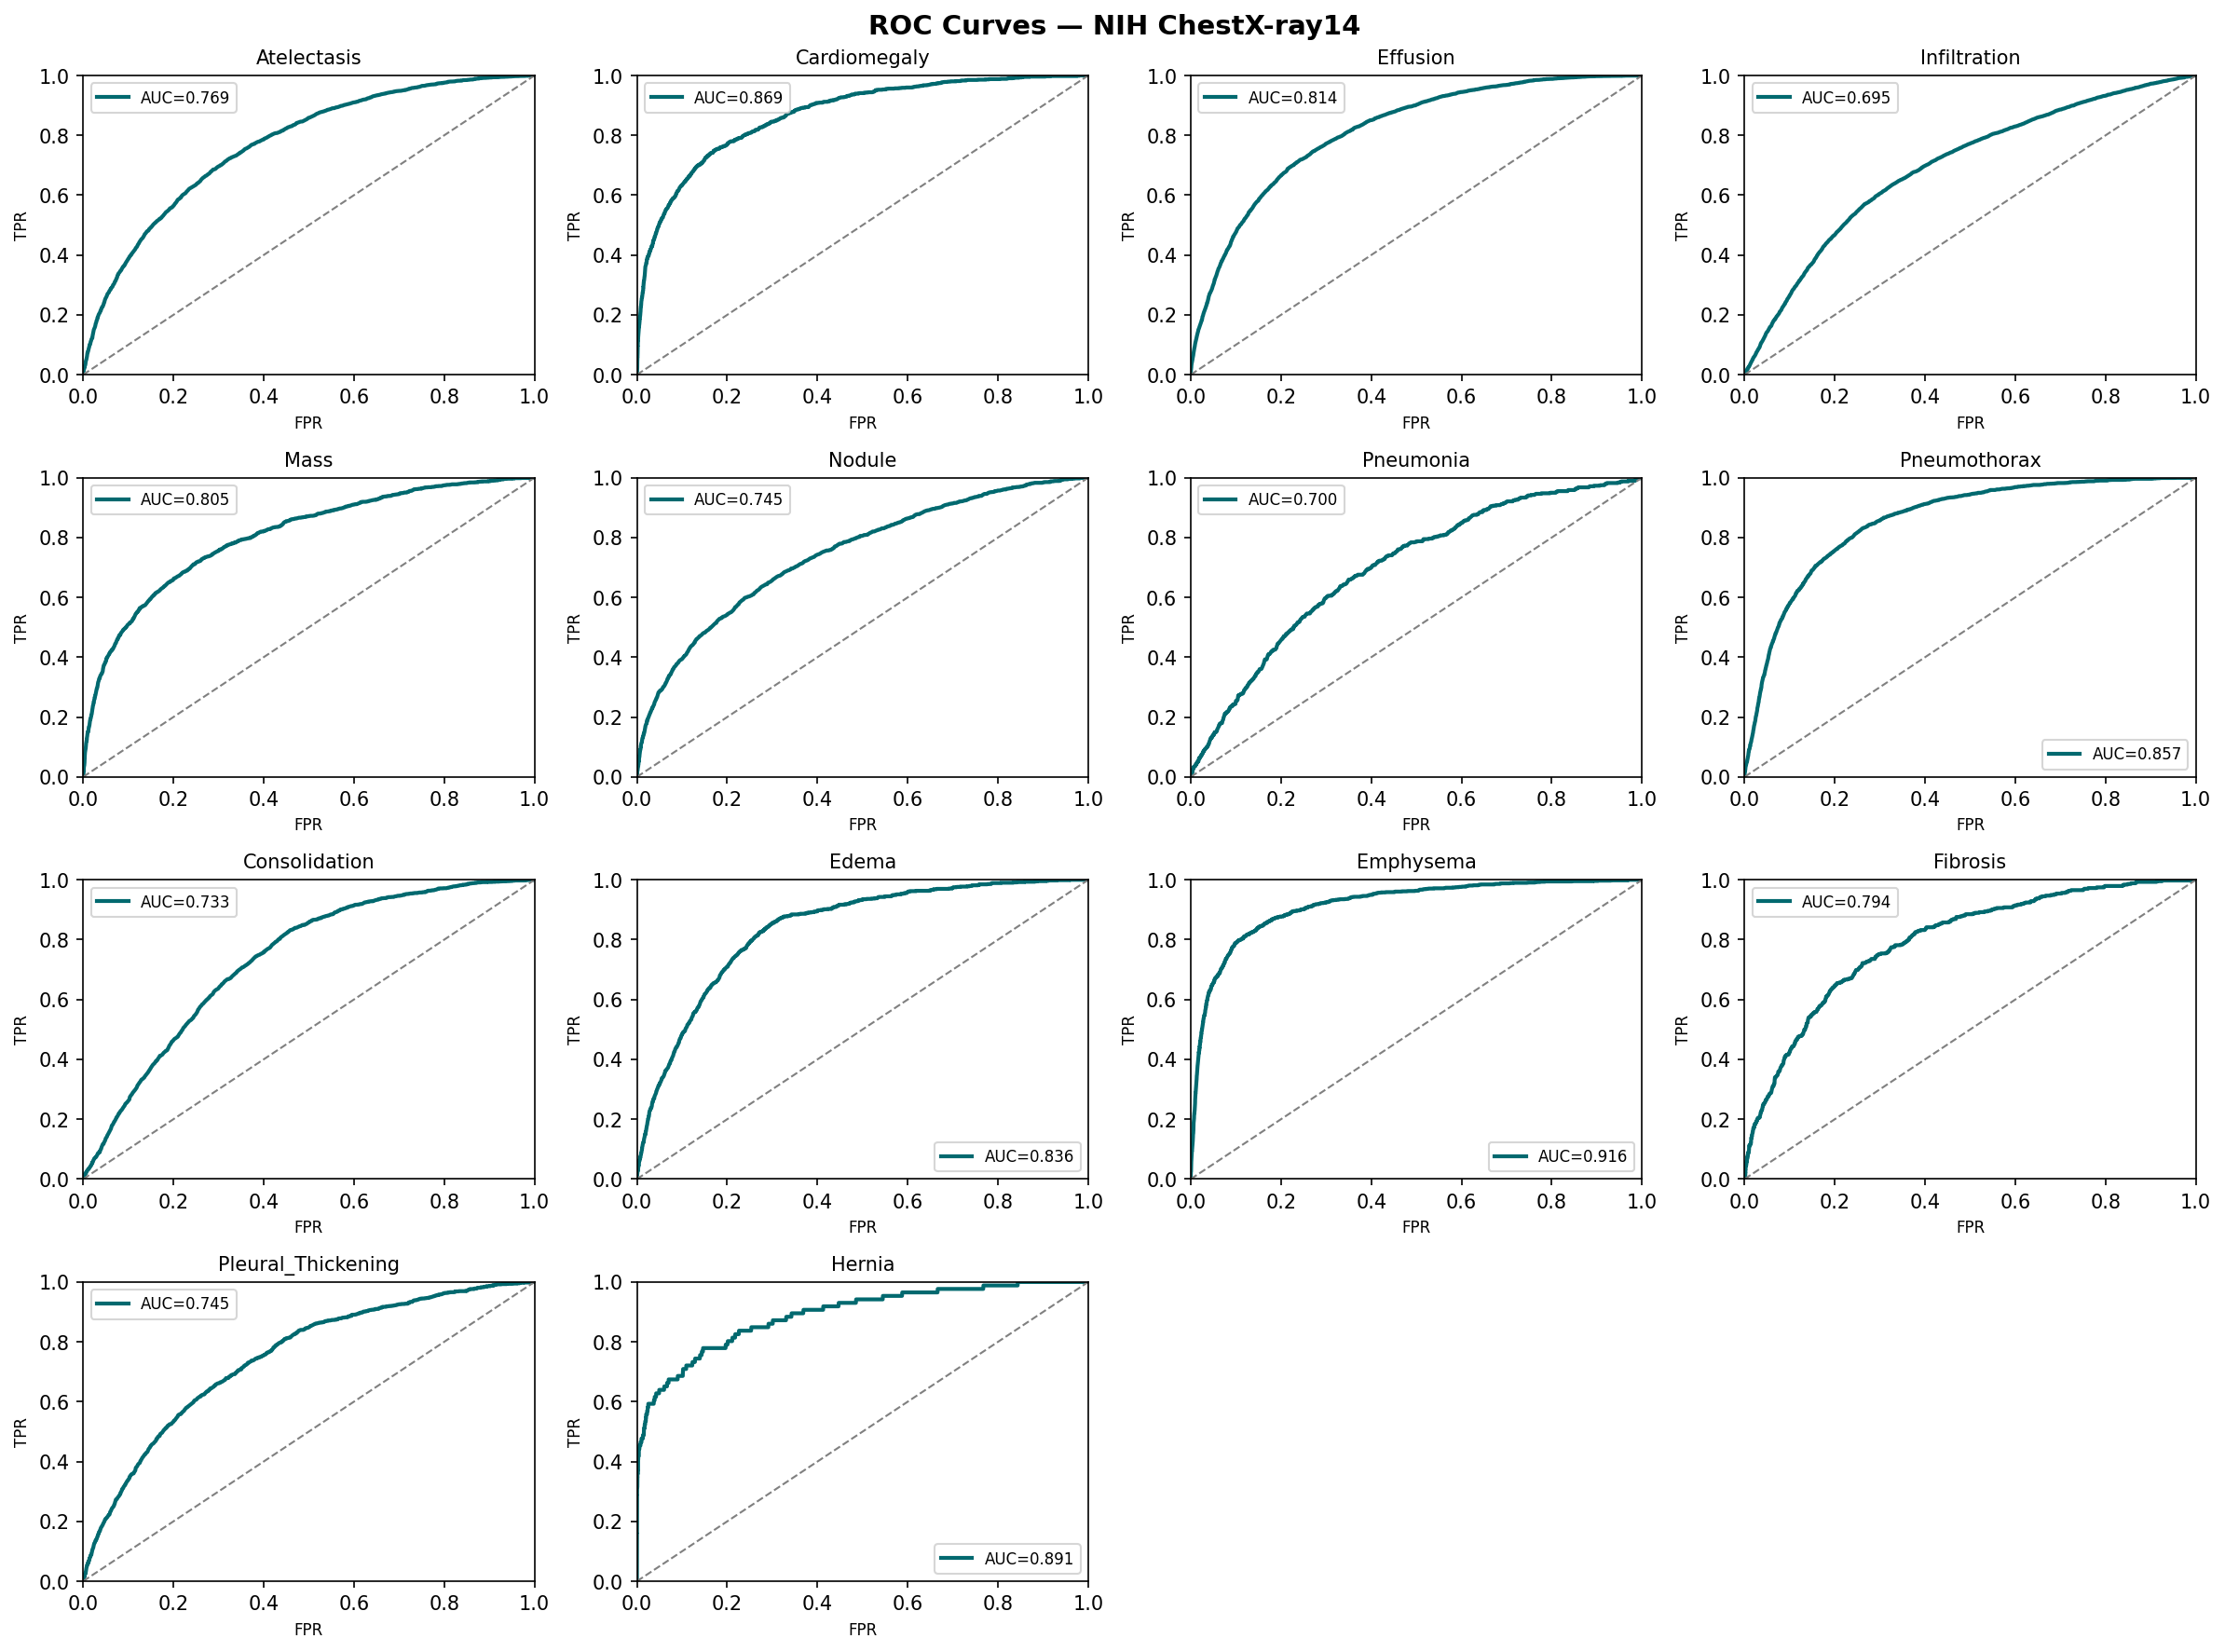
\includegraphics[width=\textwidth]{../results/figures/roc_curves_densenet121.png}
\caption{Per-class ROC curves for DenseNet-121 with Asymmetric
Loss on the ChestX-ray14 test set. Each curve represents one of
the 14 pathology classes. The diagonal line corresponds to random
performance (AUC = 0.5).}
\label{fig:roc}
\end{figure}

\subsection{Qualitative Analysis}

Grad-CAM maps computed on representative test images show
anatomically coherent attention patterns for several pathologies.
For Cardiomegaly, the model reliably highlights the cardiac
silhouette, which is the primary radiographic marker of an
enlarged heart. For Pneumothorax, activation concentrates along
the peripheral lung margins where pleural air accumulates.
For Hernia, the model attends to the diaphragmatic region,
consistent with the radiological appearance of diaphragmatic
hernias. These findings suggest the model has learned
radiologically meaningful features rather than spurious
correlates.

\begin{figure}[t]
\centering
% \includegraphics[width=\textwidth]{figures/gradcam_examples.png}
\caption{Grad-CAM activation maps for four representative
DenseNet-121 predictions. Warmer tones indicate higher importance
for the predicted class. From left to right: Cardiomegaly,
Pneumothorax, Emphysema, Hernia.}
\label{fig:gradcam}
\end{figure}

% ================================================================
\section{Discussion}
\label{sec:discussion}

The gap between DenseNet-121 and ResNet-50 in Table~\ref{tab:auc}
points to a meaningful interaction between backbone architecture
and loss function behavior on imbalanced multi-label data.
DenseNet-121's feature reuse across all layers within a dense
block creates richer and more diverse gradient pathways, which
appear to be important for learning reliable predictors for
frequent positive classes such as Atelectasis and Effusion.
ResNet-50's skip connections are more sparse by comparison and
may be insufficient to propagate the gradient signal needed for
these categories when the positive-to-negative ratio is very low.

Our mean AUC of 0.7978 sits clearly above the Wang et al.\ baseline
and is competitive with single-backbone CNN methods in the
literature, which generally fall in the 0.80 to 0.84 range on
this benchmark~\cite{ma2021vit}. The remaining gap relative to
more recent transformer-based approaches relates mainly to two
factors: the absence of explicit label dependency modeling in our
framework, and the inherent noise in ChestX-ray14 labels, which
were derived from NLP processing of radiology reports and are
known to contain a non-trivial error rate~\cite{oakden2020hidden}.
This noise sets a practical ceiling on AUC regardless of model
architecture.

\paragraph{Limitations.}
Label noise is the most significant limitation of this study.
Oakden-Rayner et al.~\cite{oakden2020hidden} have shown that
label error rates in ChestX-ray14 can be substantial for certain
categories, which complicates both training and evaluation. Beyond
label quality, the current framework treats each of the 14 classes
as conditionally independent given the image, ignoring known
clinical co-occurrence patterns such as the association between
Effusion and Consolidation. Incorporating a label correlation
module could further improve performance on co-occurring classes.

\paragraph{Future directions.}
Several extensions are planned. First, replacing the CNN backbone
with a vision transformer or hybrid CNN-ViT model could improve
capture of long-range spatial context, which is relevant for
diffuse pathologies such as Infiltration and Emphysema. Second,
validating the trained model on external datasets such as MIMIC-CXR
and CheXpert would provide a clearer picture of generalizability
beyond ChestX-ray14. Third, a systematic fairness analysis across
patient subgroups defined by sex and age would be important before
any clinical deployment, given documented disparities in AI
performance across demographic groups.

% ================================================================
\section{Conclusion}
\label{sec:conclusion}

This paper presented MedVision-AI, a multi-label chest X-ray
classification system built on DenseNet-121 and Asymmetric Loss,
augmented with Grad-CAM for visual interpretability. On the NIH
ChestX-ray14 benchmark, the system achieves a mean AUC of 0.7978,
surpassing the Wang et al.\ baseline by 6.0 points and a
comparable ResNet-50 model by 9.1 points. The backbone comparison
reveals that DenseNet-121's dense connectivity provides a
meaningful advantage over residual connections when training with
Asymmetric Loss on strongly imbalanced multi-label data. Grad-CAM
visualizations confirm that the model attends to anatomically
plausible regions for pathologies with well-defined spatial
characteristics. All code, model checkpoints, and a Gradio
deployment interface are publicly available.

% ================================================================
\bibliographystyle{splncs04}
\bibliography{references}

\end{document}
